%% PNAStwoS.tex
%% Sample file to use for PNAS articles prepared in LaTeX
%% For two column PNAS articles
%% Version1: Apr 15, 2008
%% Version2: Oct 04, 2013



%% BASIC CLASS FILE
\documentclass{pnastwo}

\setlength{\footskip}{.5in}

%% ADDITIONAL OPTIONAL STYLE FILES Font specification
\usepackage{natbib}
\usepackage{bm}% bold math
%\newcommand{\bm}[1]{\boldsymbol{#1}} %makes bold math symbols easier
\newcommand{\R}{\textsf{R}\space} %R in textsf font
\newcommand{\X}{\bm{\mathcal{X}}} %shorthand for iid
\renewcommand{\P}{\mathcal{P}}
\newcommand{\bt}{\pmb{\theta}}
\newcommand{\bl}{\pmb{\lambda}}
\newcommand{\bL}{\pmb{\Lambda}}
%\newcommand{\bG}{\pmb{\Gamma}}
\newcommand{\bh}{\pmb{\text{h}}}
\newcommand{\h}{\pmb{\text{h}}}
\usepackage{amsmath,amssymb,amsthm}
\def\citeapos#1{\citeauthor{#1}'s (\citeyear{#1})}
\DeclareMathOperator*{\argmax}{arg\,max}

%\graphicspath{{/Users/matthewjdenny/Dropbox/PINLab/Projects/Denny_Working_Directory/2011_Analysis_Output}}

%\usepackage{pnastwoF}



%% OPTIONAL MACRO DEFINITIONS
\def\s{\sigma}


\begin{document}

\title{Content-Conditioned Hierarchical Latent Space Models for Text-Valued Networks}

\author{
Matthew Denny\affil{1}{University of Massachusetts Amherst},
James ben Aaron\affil{1}{},
Hanna Wallach\affil{1}{}\affil{2}{Microsoft Research NYC},
\and Bruce Desmarais\affil{1}{},
}

\contributor{\vspace{-.25cm}}


\maketitle

\begin{article}
\begin{abstract}
{Statistical topic models are widely used to represent content in textual corpora. When documents in a corpus are attributed with senders and recipients, the corpus constitutes text-valued relational or network data. We develop a class of models for the topical content and relational structure of communications in which the rate of communication between actors is governed by covariate-conditioned latent space embeddings of the actors, and each embedding is associated with a cluster of topics. We present Markov Chain Monte Carlo methods for inference within the Bayesian framework. This model holds the potential for extensive application to real-world social and organizational relational communication data. To illustrate the model and evaluate its performance, we present an application to internal e-mail communications among managers in North Carolina county governments. We illustrate the use of covariates in the model with gender and find that patterns of gender mixing vary with the topical content of communication in a way that is consistent with the content-conditional gendered patterns that have been found to characterize social and organizational networks}
\end{abstract} 

%\keywords{weighted networks |  | x-ray reflectivity | molecular electronics}

%\abbreviations{SAM, self-assembled monolayer; OTS, octadecyltrichlorosilane}

\section{Introduction}



% general overview of the solution we will develop and immediately related recent work


\section{Results} 


\begin{tabular}{c}
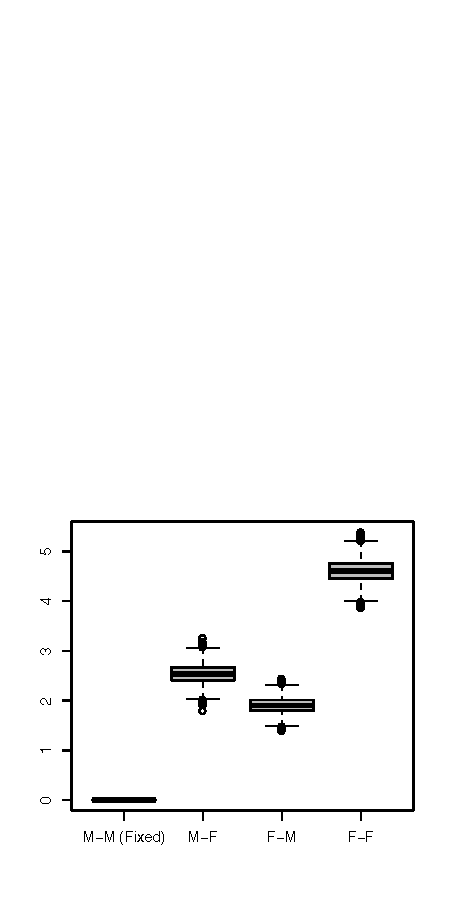
\includegraphics[width = 0.19\textwidth]{images/SS_Columbus_11-30-14_Beta1.pdf}\\
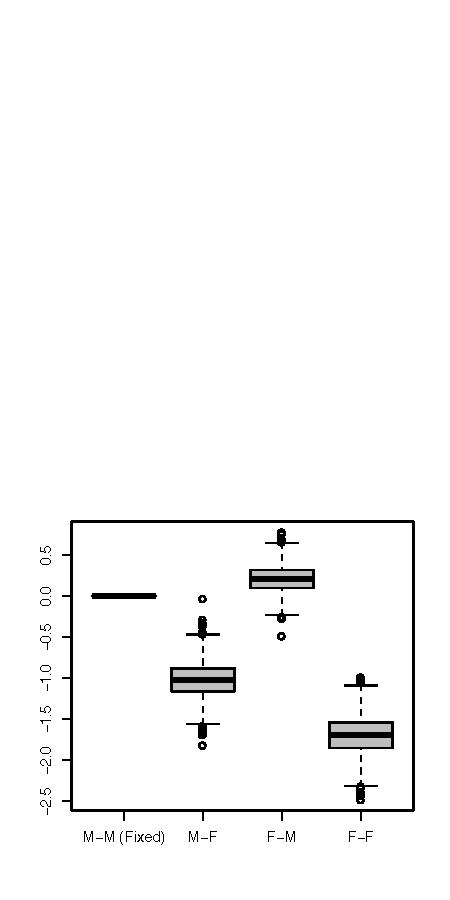
\includegraphics[width = 0.19\textwidth]{images/SS_Columbus_11-30-14_Beta10.pdf}
\end{tabular}




\end{article}



\end{document}


